\documentclass[twocolumn]{revtex4-2}

\usepackage{bm}
\usepackage{hyperref}
\usepackage{graphicx}
\usepackage{subcaption}
\usepackage{tikz}
\usetikzlibrary{arrows,shapes,snakes,automata,backgrounds,petri}

\usepackage{natbib}

\begin{document}
\title{Water Electrolysis}
\author{Sixten Nordegren}

\date{\today}

\maketitle
\section{Introduction}
Water electrolysis is the process of separating the molecules of water $H_2O$ Into it's 
constituents $H_2$ and $O_2$ gas. This is done in two separate chemical reactions the
oxidisation of water.

\begin{equation}
	2H_2O \rightarrow O_2 + 4 H^+ +4e^- 
	\label{eq: oxidisation}
\end{equation}
and the reduction of Hydrogen ions.
\begin{equation}
	2 H^+ + 2e^- \rightarrow H_2
	\label{eq: reduction}
\end{equation}

The reaction described above does not happen all by itself. An electrical feild needs to be
applied over the substance and catalysts are used to make the process happen at all. The 
thermodynamical minimum voltage that needs to be applied is $1.23 V$. 

In order to make electric charges travel through the water more effectively electrolyte is 
mixed in with it. Now what previously was a quite straight forward reaction has become quite
the intricate process that can be tested extensivly with diffrent compontents acting all by
themselves in a way that effects the production of the various gases.

\par

The usage of this method as a tool for hydrogen production has a lot of upsides. The usage
of water as a source of fuel and the only byproduct being oxygen makes the process comparably
enviromentaly freindly to it's alternatives \cite{DOSSANTOS2017563}. As of today water electolysis is responsible for about $4\%$ of the global Hydrogen
production. The reason for the quite low marketshare inspite of all the afformention upsides 
is that the process is simpy to inefficient and it's materials expensive\cite{SHIVAKUMAR2019442}.

To find a diffrent set of circumstances to make the process more efficient is currently an
active field of research. 

The aim of the experiment is to find what catalysts correlate to the most effective form of 
hydrogen and oxygen production.

\begin{figure}[t]
	\centering
	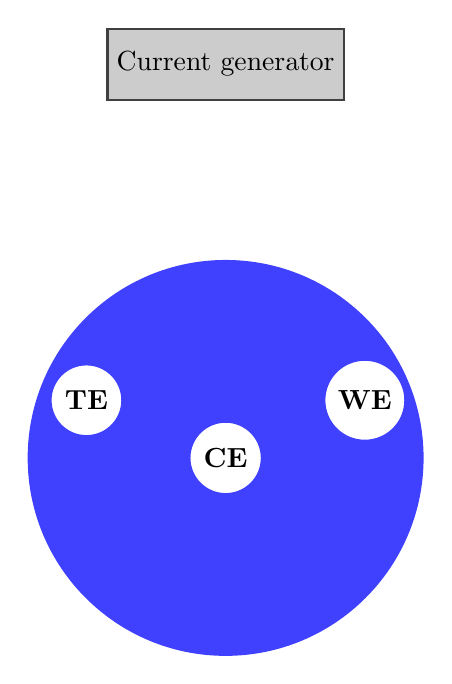
\begin{tikzpicture}[node distance = 2.5cm]
	  \tikzstyle{place}=[circle,thick,draw=blue!75,fill=white!20,minimum size=6mm]
	  \tikzstyle{red place}=[place,draw=blue!75,fill=blue!75, minimum size= 50mm]
	  \tikzstyle{transition}=[rectangle,thick,draw=black!75,
				  fill=black!20,minimum size=9mm]

		
		\node (a2) {};
		\node[red place](center) [below of =a2]  {};

		\node[transition] (a2.1) [above of =a2] {Current generator};
		\node (b1)[place] [below right of =a2] {\textbf{WE}};
		\node[place] (c1) [below of =a2] {\textbf{CE}};
		\node (b3)[place] [below left of =a2] {\textbf{TE}};

		%\draw (a2.1) -- (b1);
		%\draw (a2) -- (b3);
		%\draw (a2) -- (c1);
		
	 
	\end{tikzpicture}
\end{figure}
\section{Method}
\subsection{Catalyst testing}
Three electrodes where lowered down into water with the electrolyte mixed into it.
One Working Electorde (\textbf{WE}) from which all the measurments are made. One counter
electrode (\textbf{CE}) that was placed in the water in order to esablish a 
homogenous electric field. And lastly a final measuring electrode were inserted
into the mixture in order to make proper measurments of the wokring electorde.

\begin{figure}[b]
	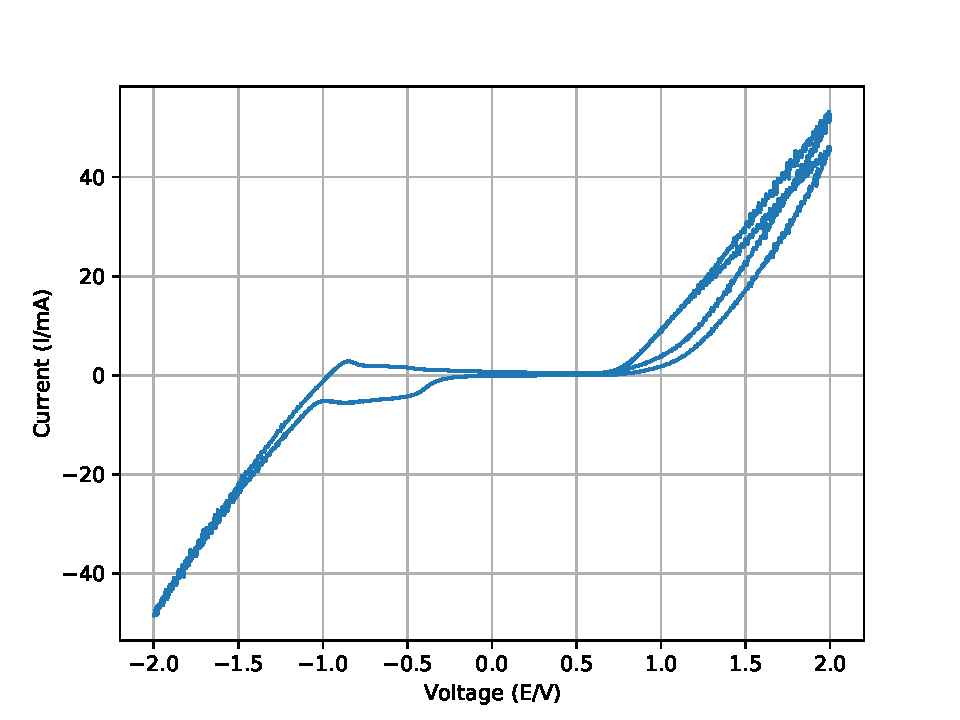
\includegraphics[width=0.9\linewidth]{/home/sixten/water_electrolysis/data_analysis/plots/data_plot_1.pdf}
	
	\caption{Plot from the first Platinum Platinum measurment \label{fig:I_Plt_1}}
\end{figure}



On the end of the \textbf{WE} and the \textbf{CE} two metals are attatched acting 
as catalysts for the chemical reaction. 

Current was sent thorught the working electrode via a current generator. Increased
from zero to a set value and working down to that same set value but with changed 
polarity.


See \ref{fig:I_Plt_1} for an example of what the procedure described above might produce.

This procedure is repeated testing diffrent metals acting as cacalytsts.

\subsection{Gas collection}
Empty tubes are lowerd down into the water resting above the catalyts and subsecquently
have their air suckedc out of them. Allowing the bubbles that ineveitably form on the
catalyts to float up into the empty tubes. 

\par 
Far from all of the gas make it into the tubes but the ammount that does are about equal
for either reaction so the gas that is infact trapped inside of the tube is representative
of the actual gas produced.

\par 
When placing down the tubes and sucking all the air out of them thre is a need to get into 
physical contact with the electrolyte. Since "ELECTROLYTE 1" is highly corrossive we change 
it out for standard $HCL$ (salt) which is a lot safer.
\par 
Instead of cycling between positive and negative polarity at eatch of the electordes. A simple 
direct current is sent through the circuit using some of the catalysts that we found 
interesting from the results from the previous experiment.
\par


\subsection{Analytical methods}
The current generator changes goes throught a set number of cycles for each measurment.
This is done in order to make minimize any random errors that might occur. Unfortionatly
each cycle wasn't exactly the same lenght as the previous one, for reasons probably only
known to the makers of the current generator, so in order to take sensible averages
some points from the longer data cycles where cropped in order to averages the cycles.
\par
The removed sections of data comes from the middle of the data sets, points that, for reasons 
that will be revealed bellow wont be used for further analysis anyway.
\par
In order to standardize the measurments we need to control for the differeing sizes of the catalysts
that where in the water. Therefore we divide each datapoint by the area of the corresponding
catalyst in order to attain the current density.
\par
We expect the relationship of the current density vs the overpotential to be of exponential
characteristic so we plot the $\bm{\log{()}} $ of a part of the data that represents the overpotential.
More details of how this is done will be included in the discussion part of the article.

\section{Results}
All the data for all the experiments can be found \href{
https://www.github.com/SixtenNordegren/Water_Electrolysis}{here} along with the code 
for some of the data analysis. Due to the magnitude of data collected I won't be able to
give each and every data set collected a fair showing. I will be presenting a selected 
sets of data.


\begin{table}[h]
\begin{tabular}{|c|c|c|c|c|}
	\hline
	& Copper & Platinum & Nickel & Gold \\
	\hline
	Width $(\text{cm})$&0.65 &0.80&0.65&0.65\\
	\hline
	Length $(\text{cm})$ &0.60&1.50&1.30&1.60\\
	\hline
	Area $(\text{cm}^2)$ &$0.66$&$1.20$&$1.04$&$0.85$\\
	\hline
\end{tabular}
	\caption{Table of measured lengts of catalyts submerged into water.\label{table: area}}
\end{table}

\begin{table}[t]
\begin{tabular}{c | c}
Material & $i_{ecd}$ $(A/cm^2)$ \\
\hline
\hline
Platinum & 2.651 \\ 

Copper & 3.875 \\ 

Gold & 1.16 \\ 

Nickel & 7.281 \\ 
\end{tabular}
	\caption{Table of current exchange current density for the hydrogen reaction\label{table: ecd_H}}
\end{table}

\begin{table}[t]
	\begin{tabular}{c|c}
		Material & $i_{ecd}$ $(A/cm^2)$ \\
		\hline
		\hline
		Platinum& -1.24\\
						 
		Copper& -1.19\\

		Gold& 0.62\\
					    
		Nickel& -0.03\\
	\end{tabular}
	\caption{Oxygen Exchange current densities\label{table: ecd_O}}
\end{table}

\begin{table}
	\begin{tabular}{c | c}
		HER & V $H_2$ (mL) \\
		\hline
		\hline
		Pt & 2 \\
		Au & 16 \\
		Co V 2 \\
	\end{tabular}
	\caption{Collected Hydrogen gas\label{table: gases}}
	
\end{table}
\begin{figure}[h]
	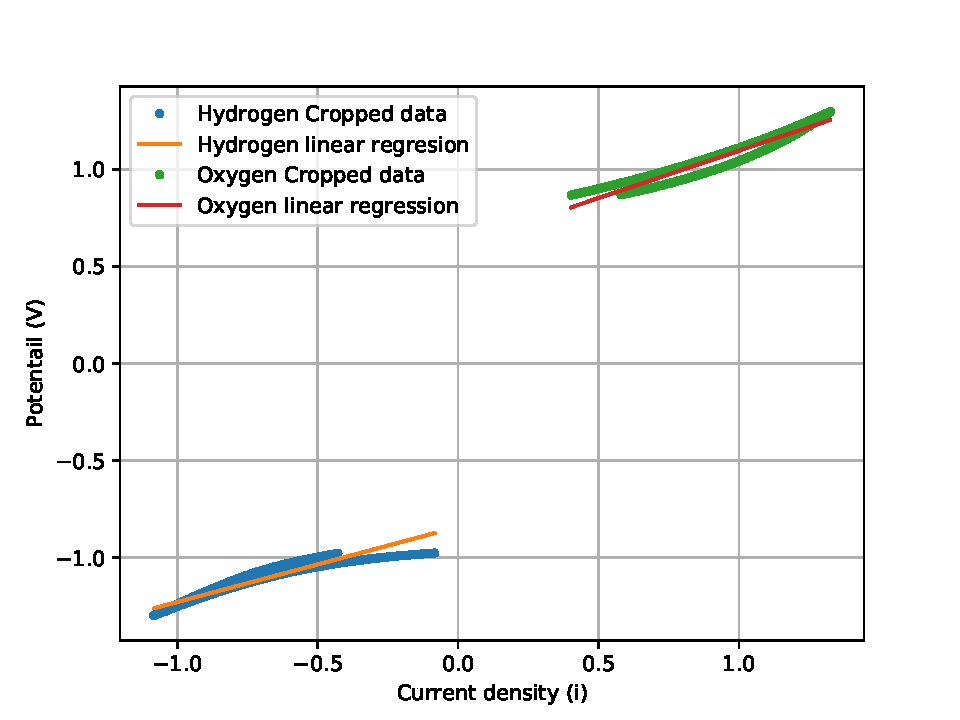
\includegraphics[width=0.95\linewidth]{/home/sixten/water_electrolysis/data_analysis/plots/Cropped_data.pdf}
	
	\caption{Logarithm of the current exchange density. With linear regression for both 
	the oxidisation and the reduction.\label{fig: CD_plat}}
\end{figure}

In table \ref{table: area} we can see the measurments of what part of the metal catalysts
that ended up in the water. This was done by extracting the catalyts after the experiment
was performed and measuring the wet parts of the catalyts with a ruler. Since the catalysts 
where hanging from cables into the water, they couldnt be held perfectly perpendicular to 
the water surface, which often resulted in a slanted mark of water on the electrode.
In those cases we simply averaged the length of the wet sides and calculated the area as 
if it was a perfect rectangles. 

\par 

\begin{figure}[h]
	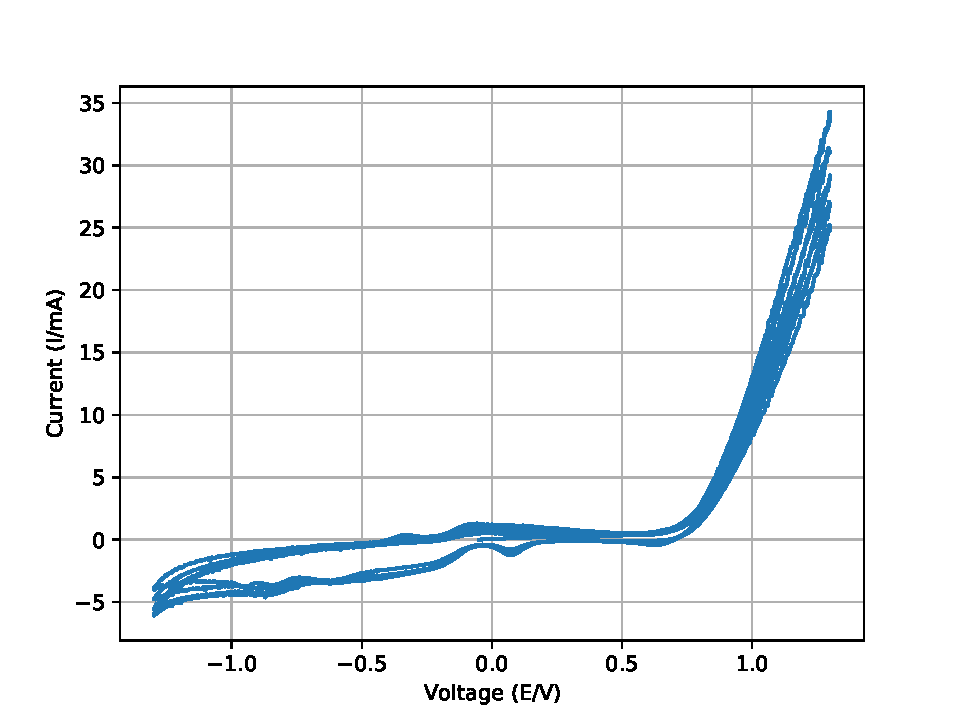
\includegraphics[width=\linewidth]{~/water_electrolysis/data_analysis/plots/data_plot_9.pdf}
	\caption{Water electrolysis with gold as the \textbf{WE}, doing a perticuarly poor job (Pt 
	is \textbf{CE})\label{figure: Au_Pt_current}}
\end{figure}

In table \ref{table: ecd_H} and \ref{table: ecd_O} we see the exchange current densities.
These values where as previously mentioned extracted by performing a linear regression on 
diffrent parts of the logarithm of measured data. This is a good method a good chunk of the 
time, but some samples are bad enough catalyts for one of the chemical reactions as not to 
barly have a reaction happen at all an example of this can be seen in figure \ref{figure: Au_Pt_current}
. Where gold is doing an almost impresivly bad job at acting as a catalyst for the hydrogen reduction
\ref{eq: reduction}. This in turn leads to some verry inacurate exchange current densities. So if 
a very perceptive reader find some of the values odd, compare to other literature values. That would
be why.

\par
The gas that was collected can be found in in table \ref{table: gases}. Originally we were supposed to 
measure the oxygen production aswell as the hydrogen production, but after  the change of electrolyte
the ammount of $O_2$ gas produced was to small in any of the reactions to produce.
\section{Discussion}
The question, what catalyst is best fitted to make either reaction as efficient as 
possible among those we tested is a rather intuative experiment by itself. The 
graphs from the initial data is already a pretty good indicator weather the catalyst
was an efective one or not. See the stark contrast between figure \ref{fig:I_Plt_1} and 
\ref{figure: Au_Pt_current}. 

\bibliography{bibliography}
\end{document}


